\documentclass{beamer}
\usepackage[utf8]{inputenc}
\usepackage[ngerman]{babel}
\usepackage{url}
\usepackage{xcolor}
\usepackage{minted}
\usepackage[absolute,overlay]{textpos}

% Defines two commands:
% * \miniframesoff -- Disable the dots in the navigation bar
% * \miniframeson -- Enables the dots in the navigation bar
\makeatletter
\let\beamer@writeslidentry@miniframeson=\beamer@writeslidentry
\def\beamer@writeslidentry@miniframesoff{%
  \expandafter\beamer@ifempty\expandafter{\beamer@framestartpage}{}% does not happen normally
  {%else
    % removed \addtocontents commands
    \clearpage\beamer@notesactions%
  }
}
\newcommand*{\miniframeson}{\let\beamer@writeslidentry=\beamer@writeslidentry@miniframeson}
\newcommand*{\miniframesoff}{\let\beamer@writeslidentry=\beamer@writeslidentry@miniframesoff}
\makeatother
% Defines an environment for latexcode
\newenvironment{latexcode}
 {\VerbatimEnvironment
  \begin{VerbatimOut}{latexcode.out}}
  {\end{VerbatimOut}%
  \inputminted[breaksymbolindentleft=2,tabsize=4]{latex}{latexcode.out}}

\newenvironment{smalllatexcode}
 {\VerbatimEnvironment
  \begin{VerbatimOut}{latexcode.out}}
  {\end{VerbatimOut}%
  \inputminted[fontsize=\scriptsize]{latex}{latexcode.out}}
% Patch fancyvrb to support unicode
% It basically \detokenize everything before writing it to a file.
\makeatletter
\newcommand{\verbments@write@detok}[1]{%
  \immediate\write\FV@OutFile{\detokenize{#1}}}
\newcommand{\verbments@FVB@VerbatimOut}[1]{%
  \@bsphack
  \begingroup
  \FV@UseKeyValues
  \FV@DefineWhiteSpace
  \def\FV@Space{\space}%
  \FV@DefineTabOut
  \let\FV@ProcessLine\verbments@write@detok
  \immediate\openout\FV@OutFile #1\relax
  \let\FV@FontScanPrep\relax
  \let\@noligs\relax
  \FV@Scan}
\let\FVB@VerbatimOut\verbments@FVB@VerbatimOut
\makeatother

\usetheme[compress]{Berlin}
\setbeamerfont{headline}{size=\large}
\setbeamerfont*{section in head/foot}{size=\tiny}
\setbeamertemplate{toc}{circle}
\setbeamertemplate{itemize subitem}[triangle] % if you want a triangle
\setbeamercovered{transparent}

\definecolor{myBlue}{rgb}{0,0.55,0.8}
\usecolortheme[named=myBlue]{structure}

\title{Das \LaTeX-KBS}
\subtitle{\small Grundlagen von \LaTeX, Ti\textit{k}Z und Co.}
\author
{
	Walter Stieben \texttt{\href{mailto:4stieben@informatik.uni-hamburg.de}{4stieben@inf}}\\
	\href{http://hauke-stieler.de/}{Hauke Stieler} \texttt{\href{mailto:4stieler@informatik.uni-hamburg.de}{4stieler@inf}}
}
\date{\footnotesize 12.01.2016}

\begin{document}
	\maketitle
	\begin{frame}
		\begin{minipage}[t][0.5\textheight]{0.5\textwidth}
			\vspace{0pt} 
			\tableofcontents
		\end{minipage}
		\begin{minipage}[t]{0.45\textwidth} 
			\vspace{0pt}  
			
\includegraphics[width=\textwidth]{./images/gib-word-keine-chance}
		\end{minipage}
	\end{frame}
		
	%%%%%%%%%%%%%%%%%%%%%%%%%%%%%%%%%%%%%%%%%%%%%%%%%%%%%%%%%%%%%%%%%%%%%%%
		
	\section{Was ist \TeX{} und \LaTeX{}}
		\subsection*{}
		\begin{frame}{Was ist \LaTeX{}}
			\textbf{\LaTeX{} und \TeX{}:}
			\begin{itemize}
				\item \TeX{} ist ein Textsatzsystem von Donald E. Knuth
				\item \LaTeX{} ist ein Satz von Makros für \TeX
				\item WYSIWYT (What You See Is What You Type)
			\end{itemize}
			\vspace{0.2cm}
			\textbf{Vorteile von \LaTeX{}:}
			\begin{itemize}
				\item Ergebnis sieht hübsch aus
				\item \LaTeX{} kümmert sich um die Formatierung
				\item Der Quelltext lässt sich Versionsverwalten
				\item Für mathematische Formeln sehr gut
				\item ``Ich möchte X mit \LaTeX{} machen'' $\rightarrow$
				Suchmaschine: ``latex X'' eingeben $\rightarrow$
				Ergebnis in den Quelltext kopieren
			\end{itemize}
		\end{frame}
		
		%%%%%%%%%%%%%%%%%%%%%%%%%%%%%%%%%%%%%%%%%%%%%%%%%%%%%%%%%%%%%%%%%%%%%%%
		
		\begin{frame}{\LaTeX{} installieren}
			\textbf{\LaTeX-Distribution:}
			\begin{description}
				\item[GNU/Linux] Nutzt den Paketmanager eurer Distribution. Debian/Ubuntu: \texttt{apt-get install texlive} 
				\item[Windows] MiKTeX herunterladen und installieren. \url{http://miktex.org/}
				\item[Mac OS] MacTex herunterladen und installieren. \url{http://tug.org/mactex/} 
			\end{description}
			\textbf{\LaTeX-Editoren:}
			\begin{description}
				\item[Kile] Guter Editor für GNU/Linux (KDE).
				\item[Gummi] Editor für GNU/Linux (GTK) mit Live-Preview
				\item[AUCTeX] für Emacs-Benutzer
				\item[Texmaker] Editor für alle Betriebssysteme
			\end{description}
			 und viele mehr \dots
		\end{frame}
		
		%%%%%%%%%%%%%%%%%%%%%%%%%%%%%%%%%%%%%%%%%%%%%%%%%%%%%%%%%%%%%%%%%%%%%%%
		
		\begin{frame}{Verschiedene \LaTeX{}-Compiler}
			Es gibt verschiedenen Compiler für \LaTeX{}. Heute: \textbf{pdflatex}
			\vspace{0.2cm}
			\textbf{Vorteile von pdflatex:}
			\begin{itemize}
				\item Direktes erzeugen einer PDF
				\item Viele PDF-Features nutzbar
				\item Einfach zu verwenden
			\end{itemize}
			\vspace{0.1cm}
			\textbf{Nachteile von pdflatex:}
			\begin{itemize}
				\item Kein \texttt{pstricks} nutzbar.
				\item Postscript-Dateien nicht direkt einbindbar
				\item Keine vollständige Unicode-Unterstützung (wie Xe\LaTeX)
			\end{itemize}
		\end{frame}
		
		%%%%%%%%%%%%%%%%%%%%%%%%%%%%%%%%%%%%%%%%%%%%%%%%%%%%%%%%%%%%%%%%%%%%%%%
		
		\begin{frame}{Detexify -- \LaTeX-Symbolerkennung}
			\begin{center}
				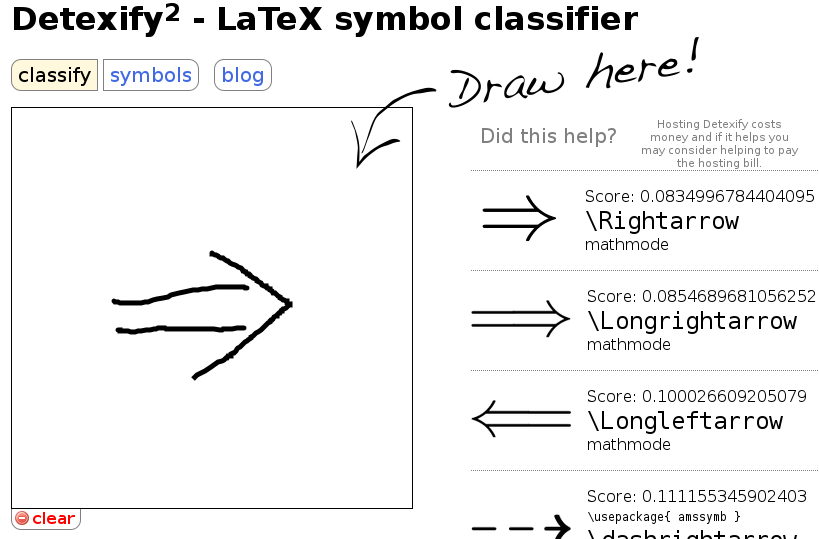
\includegraphics[width=0.95\textheight]{images/detexify}
				\vspace{0.3cm}
				
				\Large \href{http://detexify.kirelabs.org/}{http://detexify.kirelabs.org/}
			\end{center}
		\end{frame}
		
		%%%%%%%%%%%%%%%%%%%%%%%%%%%%%%%%%%%%%%%%%%%%%%%%%%%%%%%%%%%%%%%%%%%%%%%
		
		\begin{frame}{Anmerkungen}
			\textbf{Achtung:} \TeX{} ist eine Programmiersprache! Lasst nur vertrauenswürdige
			Menschen \TeX/\LaTeX-Code auf eurem Rechner/Server ausführen.
			
			\vspace{0.2cm}
			\textbf{Anmerkung:} Wenn du dir diese Folien anschaust, ist das System
			nicht mehr online. Es war nur zum Ausprobieren während des
			KunterBuntenSeminars gedacht.
		\end{frame}
		
		%%%%%%%%%%%%%%%%%%%%%%%%%%%%%%%%%%%%%%%%%%%%%%%%%%%%%%%%%%%%%%%%%%%%%%%
		
		\section{Textsatz-Grundlagen mit \LaTeX{}}
		\subsection*{}
		
		\begin{frame}{Dokumentenklassen}
			\begin{itemize}
				\item Die Dokumentenklasse beschreibt wie ein Dokument aussieht
				\item Ihr beschreibt was ihr schreibt (z.\,B. was eine Überschrift ist)
				\item \LaTeX{} formatiert euer Dokument mit Hilfe der Dokumentenklasse, nicht ihr!
			\end{itemize}
			\vspace{0.2cm}
			Beispiele für Dokumentenklassen:
			\begin{description}
				\item[Scrartcl/article:] Artikel im Umfang von mehreren Seiten
				\item[Scrllr2/letter:] Briefe
				\item[Scrreprt/report:] Reports, Umfang mehr als 15 Seiten
				\item[Scrbook/book:] Bücher
			\end{description}
		\end{frame}
		
		%%%%%%%%%%%%%%%%%%%%%%%%%%%%%%%%%%%%%%%%%%%%%%%%%%%%%%%%%%%%%%%%%%%%%%%
		
		\begin{frame}[containsverbatim]{Mein erstes Dokument}
			\begin{latexcode}
\documentclass[a4paper,10pt]{scrartcl}
\usepackage[utf8]{inputenc}
\usepackage[T1]{fontenc}
\usepackage[ngerman]{babel}
\usepackage{lmodern}

\author{Max Mustermann}
\title{Mein erstes Dokument}

\begin{document}
\maketitle{}
Hello World!
\end{document}
			\end{latexcode}
			\begin{textblock}{10}(7.5,10.5)
				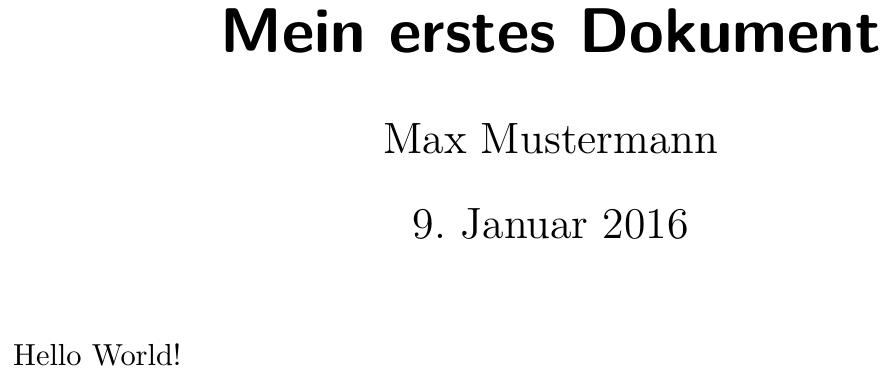
\includegraphics[width=5.5cm]{images/erstes-dokument}
			\end{textblock}
		\end{frame}
\end{document}